\section{Certified Interior Realization}\label{sec:certified}

The preceding results are analytic and do not depend on numerical sampling. We nevertheless record one certified interior realization to show that the open ecological region can be reached with nondegenerate coexistence densities and comfortable separation from both the classical and fractional boundaries.

We use \(\alpha=0.9\) and the parameter set in Table~\ref{tab:w2a}. This realization was selected from a search over constructive embeddings only after the theorem package had been fixed; the search therefore chooses a readable interior witness rather than supplying evidence for the theorem.

\begin{table}[!htbp]
\centering
\caption{Canonical certified realization W2-A. All parameters are positive; the conversion efficiencies satisfy \(0<e_1,e_2,e_3<1\).}
\label{tab:w2a}
\begin{tabular}{cccccc}
\toprule
Parameter & Value & Parameter & Value & Parameter & Value\\
\midrule
\(\alpha\) & \(0.9\) &
\(a\) & \(0.229\) &
\(K\) & \(1.4913425743\)\\
\(r\) & \(7.8104480113\) &
\(m\) & \(0.511\) &
\(h\) & \(0.1404219270\)\\
\(q_1\) & \(0.5121684678\) &
\(q_2\) & \(3.2338213736\) &
\(c_1\) & \(0.065\)\\
\(c_2\) & \(0.0509\) &
\(e_1=e_3\) & \(0.773\) &
\(e_2\) & \(0.01404592165\)\\
\(\mu_1\) & \(0.3178535346\) &
\(\mu_2\) & \(0.1209173583\) &
 & \\
\bottomrule
\end{tabular}
\end{table}

At \(m=0.511\), interval evaluation gives a well-balanced positive coexistence point and a robust interior invariant margin:
\begin{align}
 (X,Y,Z)&=(1,\;0.7856328169\ldots,\;0.1921819373\ldots),\label{eq:w2a-densities}\\
 s&=0.8231,\qquad \beta=(4.79,\;4.506,\;5.607),\qquad \kappa=62.735,\label{eq:w2a-invariants}\\
 T_1(\beta)&=44.6123995333883\ldots,\qquad
 T_{0.9}(\beta)=94.5719074446105\ldots,\\
 \kappa-T_1(\beta)&\ge18.1226004666,\qquad
 T_{0.9}(\beta)-\kappa\ge31.8369074446.\label{eq:w2a-margins}
\end{align}
The largest-to-smallest coexistence density ratio is approximately \(5.20\), and both certified margins place the point well inside the fractional-only band. The equilibrium is strictly biologically feasible (\(X,Y,Z>0\) and \(m<X<K\)); since the equilibrium equation has a simple root here, the implicit-function theorem preserves a nearby feasible equilibrium and the strict invariant margins under sufficiently small parameter perturbations.

\subsection{Interval Certification along the Allee Branch}

The coexistence branch was enclosed with the outward-rounded \texttt{mpmath.iv} interval backend. Parameter-box and equilibrium evaluations used 50 decimal digits; the scalar equilibrium equation~\eqref{eq:scalar-equilibrium} was contracted by interval Newton evaluation, and the contracted state interval was propagated through \(Y,Z,s,\beta,\kappa\) and Cain's threshold. Crucially, uniqueness of the threshold minimizer alone would \emph{not} validate a numerical lower bound. We therefore use 40-decimal-digit interval arithmetic to enclose a high-precision Newton candidate \(\widehat y\) for the minimizer of the log-objective \(G_{\alpha,\beta}\) in Equation~\eqref{eq:logobjective}. A subdivided box around \(\widehat y\) is checked for a strictly positive interval lower bound \(\underline\lambda\) on the Hessian's smallest eigenvalue (via Gershgorin or determinant-over-trace), and the gradient enclosure bounds the optimizer displacement by \(\rho_y=\overline{\|\nabla G(\widehat y)\|}/\underline\lambda\). The global strict-convexity theorem and the localization test place the true minimizer inside this box. An outward-rounded validated lower bound is then
\[
 \underline T_\alpha
 =\exp\!\Bigl(\underline{G_{\alpha,\beta}(\widehat y)}
 -\overline{\|\nabla G_{\alpha,\beta}(\widehat y)\|}\,\rho_y\Bigr)
 \le T_\alpha(\beta).
\]
For interval parameter boxes, we take the componentwise lower corner \(\underline\beta\), using monotonicity of \(T_\alpha\) in each \(\beta_{ij}\), and certify \(\underline T_\alpha(\underline\beta)-\overline\kappa>0\). As an independent check, simplex boundary-strip exclusion combined with interval branch-and-bound gives the same conclusion. The certificate thus requires both the analytic convexity result and explicit interval Hessian, gradient, and threshold enclosures; it is not inferred from an approximate optimizer.

A subdivision of the branch into 42 boxes was certified without failure on
\begin{equation}
 0.394\le m\le0.578,
 \label{eq:certified-m-range}
\end{equation}
with the strict inequalities \(\kappa-T_1>0\) and \(T_{0.9}-\kappa>0\) on every box. The smallest certified lower margins over the complete interval were \(0.0332\) and \(1.342\), respectively. The classical boundary was solved independently at
\begin{equation}
 m_0\approx0.374451281242515,
 \label{eq:w2a-m0}
\end{equation}
The unrounded high-precision computation of the Cain-gap equation used 60 decimal digits and returned a residual below \(10^{-59}\); this residual pertains to the full internal approximation, not to the shortened printed number. This agrees with Theorem~\ref{thm:crossing}.

\begin{figure}[!htbp]
\centering
\includegraphics[width=0.95\textwidth]{fig07_certified_anchor.pdf}
\caption{The three-species double-Allee intraguild-predation witness W2-A at order \(\alpha=0.9\) and anchor Allee parameter \(m=0.511\). \textbf{(a)} The positive coexistence densities \(X,Y,Z\) along the threshold branch (anchor approximately \((1,0.786,0.192)\)). \textbf{(b)} Invariant gaps \(\kappa-T_1(\beta)\) (non-Hurwitz \(D\)-stability) and \(T_{0.9}(\beta)-\kappa\) (all-diagonal Matignon stability); only the marked lower bounds and green interval are interval-certified. \textbf{(c)} Eigenvalues at the positive diagonal ratio \(D_*\) selected by scale-invariant numerical angular search; the plotted spectrum is numerical corroboration, not the all-diagonal proof.}
\label{fig:certified-anchor}
\end{figure}

\subsection{Scale-Invariant Spectral Corroboration}

As an independent numerical check, we minimized the smallest eigenvalue angle over positive diagonal ratios after fixing the geometric mean of the diagonal entries to one. This normalization is essential: raw spectral abscissa is not scale invariant under common multiplication of \(D\).

For the anchor, the most restrictive diagonal ratio found was approximately
\[
 D_*=\diag(0.1810,\;2.0474,\;2.6985),
 \qquad
 \spec(D_*B)=\{0.04494\pm0.57743i,\,-0.50930\},
\]
and
\[
 \min_j|\arg\lambda_j(D_*B)|=1.49312\ldots>0.9\frac{\pi}{2},
\]
while the conjugate pair has positive real part. Here \(B=DF(u^*)\) is the reduced per-capita derivative and \(J=\diag(u^*)B\) is the Jacobian of the \emph{unscaled} nonlinear system. The search uses a selected member \(D_*B\) of the positive-diagonal orbit, not necessarily \(J\) itself. Failure of Hurwitz \(D\)-stability means that \(\exists D\succ0\) with \(\spec(DB)\not\subset\{\Re z<0\}\), and does not assert that the unscaled \(J\) is unstable. The corresponding angular margin is about \(0.0794\) radians for \(\alpha=0.9\), whereas the classical \(\alpha=1\) margin is negative. This direct search corroborates both sides of the classification, but it is not used in the proof.

\subsection{Full Nonlinear Time-Domain Case Study}

We now integrate the complete nonlinear ecological system rather than its linearization. Let \(u=(x,y,z)^\top\), let \(u^*=(X,Y,Z)^\top\) be the anchor in Equation~\eqref{eq:w2a-densities}, and denote the unscaled nonlinear vector field in Equation~\eqref{eq:igp-model} by \(G(u)\). To realize exactly the orbit point above, set
\begin{equation}
 R_*=D_*\diag(u^*)^{-1}
 =\diag(0.1810024,\;2.6060229,\;14.0412352)
 \label{eq:row-rate-scaling}
\end{equation}
and consider the positively row-scaled model
\begin{equation}
 \CapD{\alpha}u=R_*G(u).
 \label{eq:scaled-nonlinear-case}
\end{equation}
The scaling changes only the three positive response rates, preserves the coexistence equilibrium and the interaction signs, and gives the exact Jacobian identity
\[
 R_*J=R_*\diag(u^*)B=D_*B.
\]
The \emph{unscaled} ecological model has Jacobian \(J=\diag(u^*)B\); for the comparison we explicitly choose the positive response-rate configuration \(R_*\), whose Jacobian is \(R_*J=D_*B\). This selected row-scaled nonlinear model has a locally Matignon-stable equilibrium at \(\alpha=0.9\) and a classically unstable equilibrium at \(\alpha=1\). All-diagonal Matignon stability is a separate analytic statement.

Both integrations start from the identical relative perturbation
\[
 u(0)=u^*\odot\bigl(\mathbf 1+10^{-3}(1,-1,1)^\top\bigr)
      =(1.001,\;0.7848471840,\;0.1923741192)^\top.
\]
For \(\alpha=0.9\), we used the fractional Adams--Bashforth--Moulton PECE method \cite{Garrappa2010,Garrappa2018,Diethelm2010} with \(h=0.01\) on \(0\le t\le180\). Step halving gave maximum componentwise relative differences of \(1.15\times10^{-6}\) between \(h=0.04\) and \(0.02\), and \(3.14\times10^{-7}\) between \(h=0.02\) and \(0.01\), an observed refinement order of \(1.875\). The relative distance \(\|u/u^*-\mathbf 1\|_2\) decreased from \(1.732\times10^{-3}\) to \(7.97\times10^{-6}\), and all three states remained positive.

For \(\alpha=1\), an adaptive DOP853 integration with relative and absolute tolerances \(10^{-11}\) and \(10^{-13}\), respectively, was stopped when the same relative distance first reached \(0.2\). This occurred at \(t=101.586\), consistent with the positive real part of the conjugate pair. Stopping at the declared radius keeps the comparison within a fixed local neighborhood; it is not a claim about the global fate of the classical trajectory.

\paragraph{Long-horizon nonlinear Caputo verification across the exact boundary order.}
The four-invariant threshold defines the boundary order \(\alpha_*\) by
\(T_{\alpha_*}(\beta)=\kappa\). The extremal positive diagonal obtained
independently from the angular search satisfies, at the displayed precision,
\[
 \alpha_* =0.9505501071\ldots
 =\frac{2}{\pi}\min_j|\arg\lambda_j(D_*B)| .
\]
This is the critical order of the selected row-scaled
Jacobian \(R_*J=D_*B\). With the same W2-A model, positive response rates
and initial perturbation, an additional sweep of the \emph{full nonlinear}
Caputo equations covered \(0.7\le\alpha\le1\), including a dense grid
with \(\Delta\alpha=0.001\) and additional points around \(\alpha_*\).
The Adams--Bashforth--Moulton PECE runs used \(h=0.02\) and
\(h=0.01\) for step refinement. The horizon was \(t=600\) away from
the boundary and was extended to \(t=2000\) near it
(\(|\alpha-\alpha_*|<0.02\)). Integration was terminated when the
relative distance \(d(t)=\|u(t)/u^*-\mathbf1\|_2\) first reached
the declared local-neighborhood radius \(0.2\);
an independent DOP853 integration at \(\alpha=1\) reproduced
the integer-order exit time.

Table~\ref{tab:order-scan} summarizes representative orders.
For non-exiting trajectories, the late rate is the fitted
finite-window slope of \(\log d(t)\) over the last half
of the integration, not an asymptotic exponential-decay
exponent for fractional dynamics.
Negative and positive fitted rates on either side of
\(\alpha_*\) corroborate the local spectral classification.
The near-critical order \(\alpha=0.9506\) illustrates
the danger of classifying solely by final versus initial distance:
its late rate is positive, but
\(d(2000)=1.322\times10^{-3}<d(0)=1.732\times10^{-3}\).
The unscaled configuration \(R=I\) has a Hurwitz Jacobian and
decayed at all tested orders.

\begin{table}[!htbp]
\centering
\caption{Long-horizon full nonlinear W2-A Caputo order sweep near
the predicted order boundary \(\alpha_*=0.9505501071\ldots\),
with fixed positive row scaling \(R_*\).
All runs share the same \(10^{-3}(1,-1,1)\) relative initial
perturbation. The PECE method uses \(h=0.01\) with refinement
against \(h=0.02\), terminating at radius \(d=0.2\).
The late rate (units \(10^{-3}\)) is a fitted
finite-time slope of \(\log d(t)\); a dash means that the
trajectory exited and was stopped.
Exit time is the first occurrence of \(d=0.2\).
The numerical experiment corroborates but does not prove
the analytic spectral boundary.}
\label{tab:order-scan}
\begin{tabular}{ccccc}
\toprule
\(\alpha\) & \(t_{\mathrm{end}}\) & \(d(t_{\mathrm{end}})\) &
late rate \((10^{-3})\) & exit time \\
\midrule
\(0.9000\) & \(600\) & \(2.574\times10^{-6}\) & \(-2.075\) & ---\\
\(0.9450\) & \(2000\) & \(3.570\times10^{-7}\) & \(-3.531\) & ---\\
\(0.9500\) & \(2000\) & \(3.253\times10^{-4}\) & \(-0.509\) & ---\\
\(0.9506\) & \(2000\) & \(1.322\times10^{-3}\) & \(+0.046\) & ---\\
\(0.9510\) & \(2000\) & \(3.588\times10^{-3}\) & \(+0.417\) & ---\\
\(0.9520\) & \(2000\) & \(3.227\times10^{-2}\) & \(+1.347\) & ---\\
\(0.9530\) & \(2000\) & \(0.200\) & --- & \(1955.0\)\\
\(0.9550\) & \(2000\) & \(0.200\) & --- & \(1084.0\)\\
\(1.0000\) & \(600\) & \(0.200\) & --- & \(101.6\)\\
\bottomrule
\end{tabular}
\end{table}

Figure~\ref{fig:alpha-sweep} displays trajectories and the
late-rate sign change around the theoretically predicted order.
In total, the two-stage sweep comprised 363 integrations.
The end-versus-start distance diagnostic agreed with the
linear spectral prediction in 339 of 340 dense runs;
the sole near-critical exception has a positive late fitted
rate but has not yet recovered its initial distance by \(t=2000\).
This is finite-horizon numerical corroboration, not an
independent proof of fractional asymptotic stability.

\begin{figure}[!htbp]
\centering
\includegraphics[width=0.96\textwidth]{fig09_nonlinear_caputo_dynamics.pdf}
\caption{Full nonlinear time-domain comparison at the positive coexistence equilibrium of W2-A, with the selected positive response-rate scaling \(R_*\). \textbf{(a)} Relative deviations \(u_i(t)/u_i^*-1\) for each species at Caputo order \(\alpha=0.9\), computed with PECE step \(h=0.01\), showing damped oscillations. \textbf{(b)} Relative Euclidean distance \(\|u(t)/u^*-\mathbf1\|_2\) comparing \(\alpha=0.9\) against integer-order \(\alpha=1\), with identical parameters and initial state; the classical DOP853 trajectory ends upon reaching radius \(0.2\). The comparison concerns local dynamics, not global attraction.}
\label{fig:nonlinear-caputo-dynamics}
\end{figure}

\begin{figure}[!htbp]
\centering
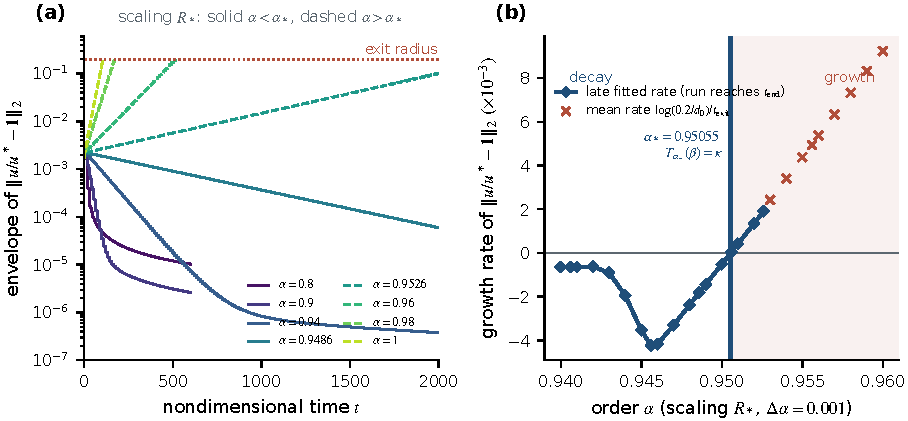
\includegraphics[width=0.97\textwidth]{fig10_alpha_sweep.pdf}
\caption{Full nonlinear three-species W2-A Caputo dynamics across
the order boundary \(\alpha_*=0.9505501071\ldots\)
for the fixed positive row-rate configuration \(R_*\).
\textbf{(a)} Running-window envelope of relative
coexistence distance
\(d(t)=\|u(t)/u^*-\mathbf1\|_2\) versus nondimensional time
for selected fractional orders on either side of the boundary;
the dotted horizontal line marks the stopping radius \(d=0.2\).
\textbf{(b)} Late fitted log-distance rate versus order \(\alpha\)
near the boundary. Diamonds are uninterrupted PECE integrations;
crosses denote trajectories stopped at the exit radius and plot
the mean rate \(\log(0.2/d(0))/t_{\mathrm{exit}}\) instead.
The vertical line is the analytic threshold
\(T_{\alpha_*}(\beta)=\kappa\), not fitted to the trajectories.
The simulations use PECE \(h=0.01\) with refinement
at \(h=0.02\). The boundary follows from the theorem;
the drawn trajectories and rates are finite-horizon
numerical corroboration.}
\label{fig:alpha-sweep}
\end{figure}

Finally, Figure~\ref{fig:ecological-contrast} places the exact two-dimensional equality curve beside the three-dimensional open region. In panel (b), the region boundaries are traced by deterministic root finding applied to the exact formulas. The traced regions themselves are pointwise formula evaluations; only the green segment and marked anchor carry interval-certification semantics.

\begin{figure}[!htbp]
\centering
\includegraphics[width=0.96\textwidth]{fig08_double_allee_2d_3d.pdf}
\caption{Geometric double-Allee contrast. \textbf{(a)} In the two-species model the fractional-only set in prey-equilibrium \(X\) versus Allee threshold \(m\) is the codimension-one curve \(m=m_c(X)\). \textbf{(b)} For the three-species W2-A model at \(\alpha=0.9\), the \((m,K)\) plane contains the classical Cain boundary \(\kappa=T_1\), the fractional Matignon boundary \(\kappa=T_{0.9}\), and the feasibility edge, enclosing an open fractional-only region. Curves and filled regions come from numerical evaluations of the exact formulas; only the indicated green interval is rigorously enclosed.}
\label{fig:ecological-contrast}
\end{figure}
